\chapter{Detecting corruption, collusion \& fraud: Data product}\label{chap_product}

\section{Data pipeline}
\begin{figure}[H]
\begin{center}
\caption{Data pipeline}
\label{fig_pipeline}
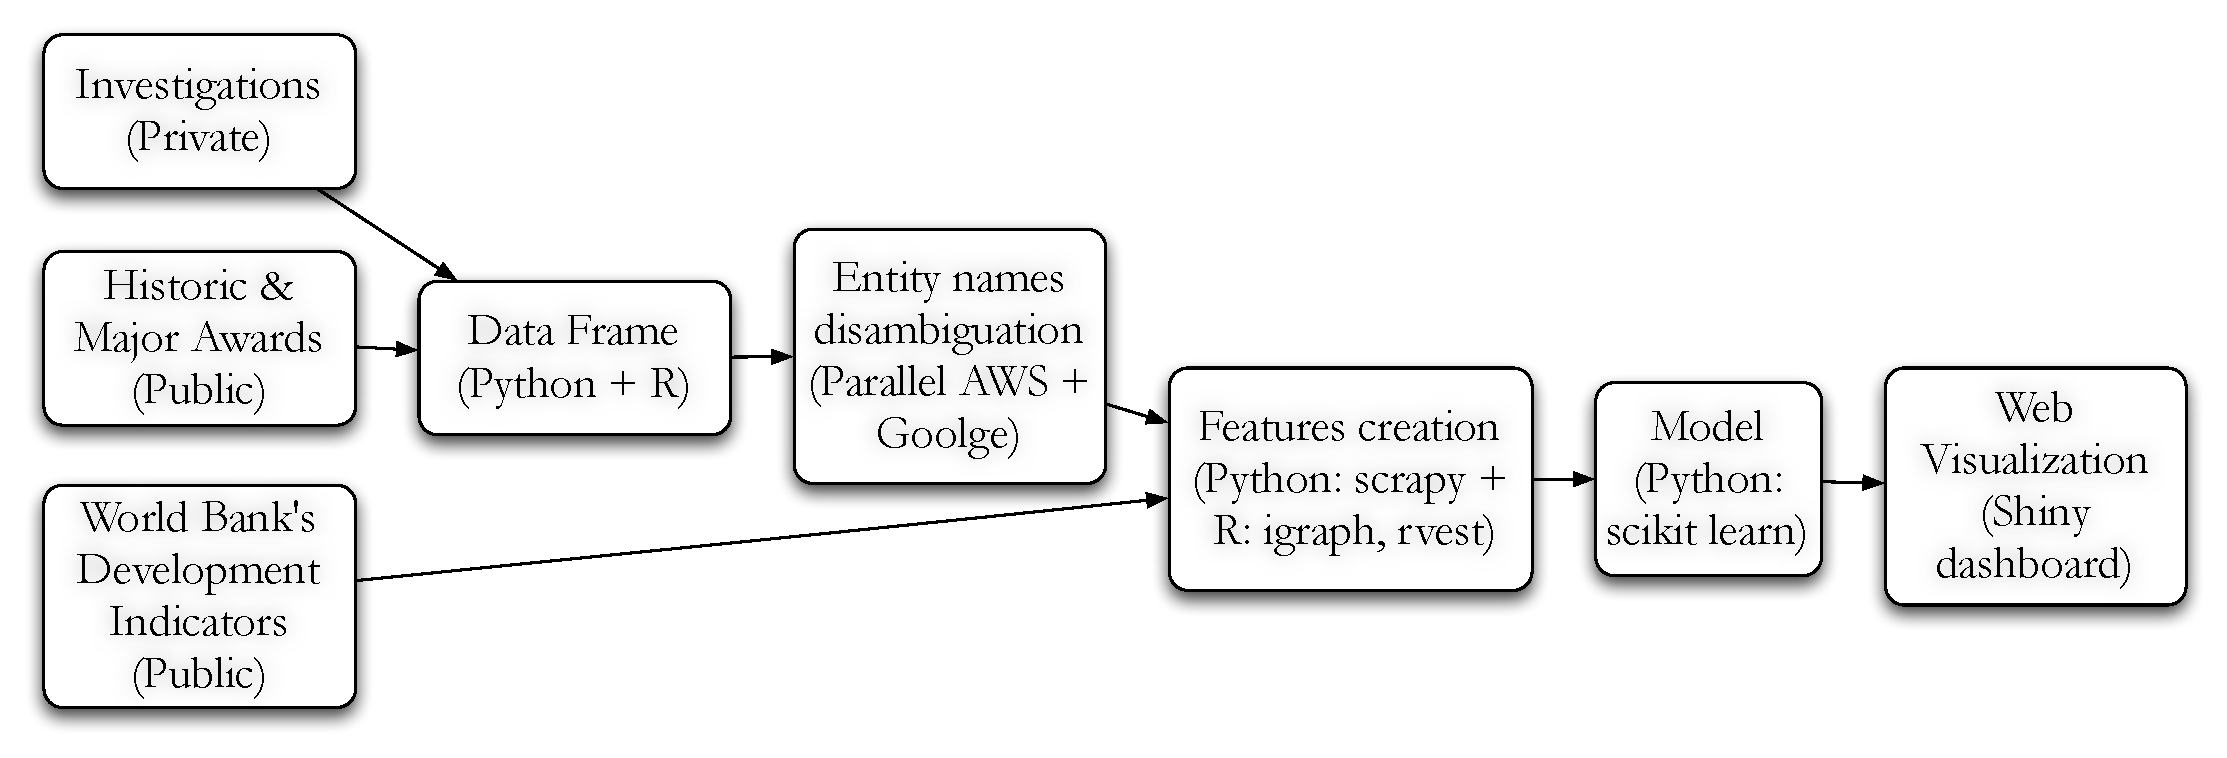
\includegraphics[width=\textwidth,height=1\textheight,keepaspectratio]{../img/pipeline.pdf}
\end{center}
\noindent \footnotesize{\textbf{Source:} Own creation.}
\end{figure}

\section{Red-flags from data}

Chapter \ref{chap_procurements} presented figure \ref{fig_what_corr} suggesting ideas of how to look for common patterns to identify potential cases of corruption, collusion, fraud, coercion and other types of malicious behavior among the procurements that the World Bank gives to countries all over the world. The objective of this section is to try to replicate those figures by using real data in order to provide a valuable insight to the investigators working in the Integrity Vice Presidency to help them attack this problem.



\section{Model}

\section{Web visualization application: dashboard}

\subsection{Dashboard outline}

\subsection{Interactive map}

\begin{figure}[H]
\begin{center}
\caption{Interactive map}
\label{fig_interactive_map}
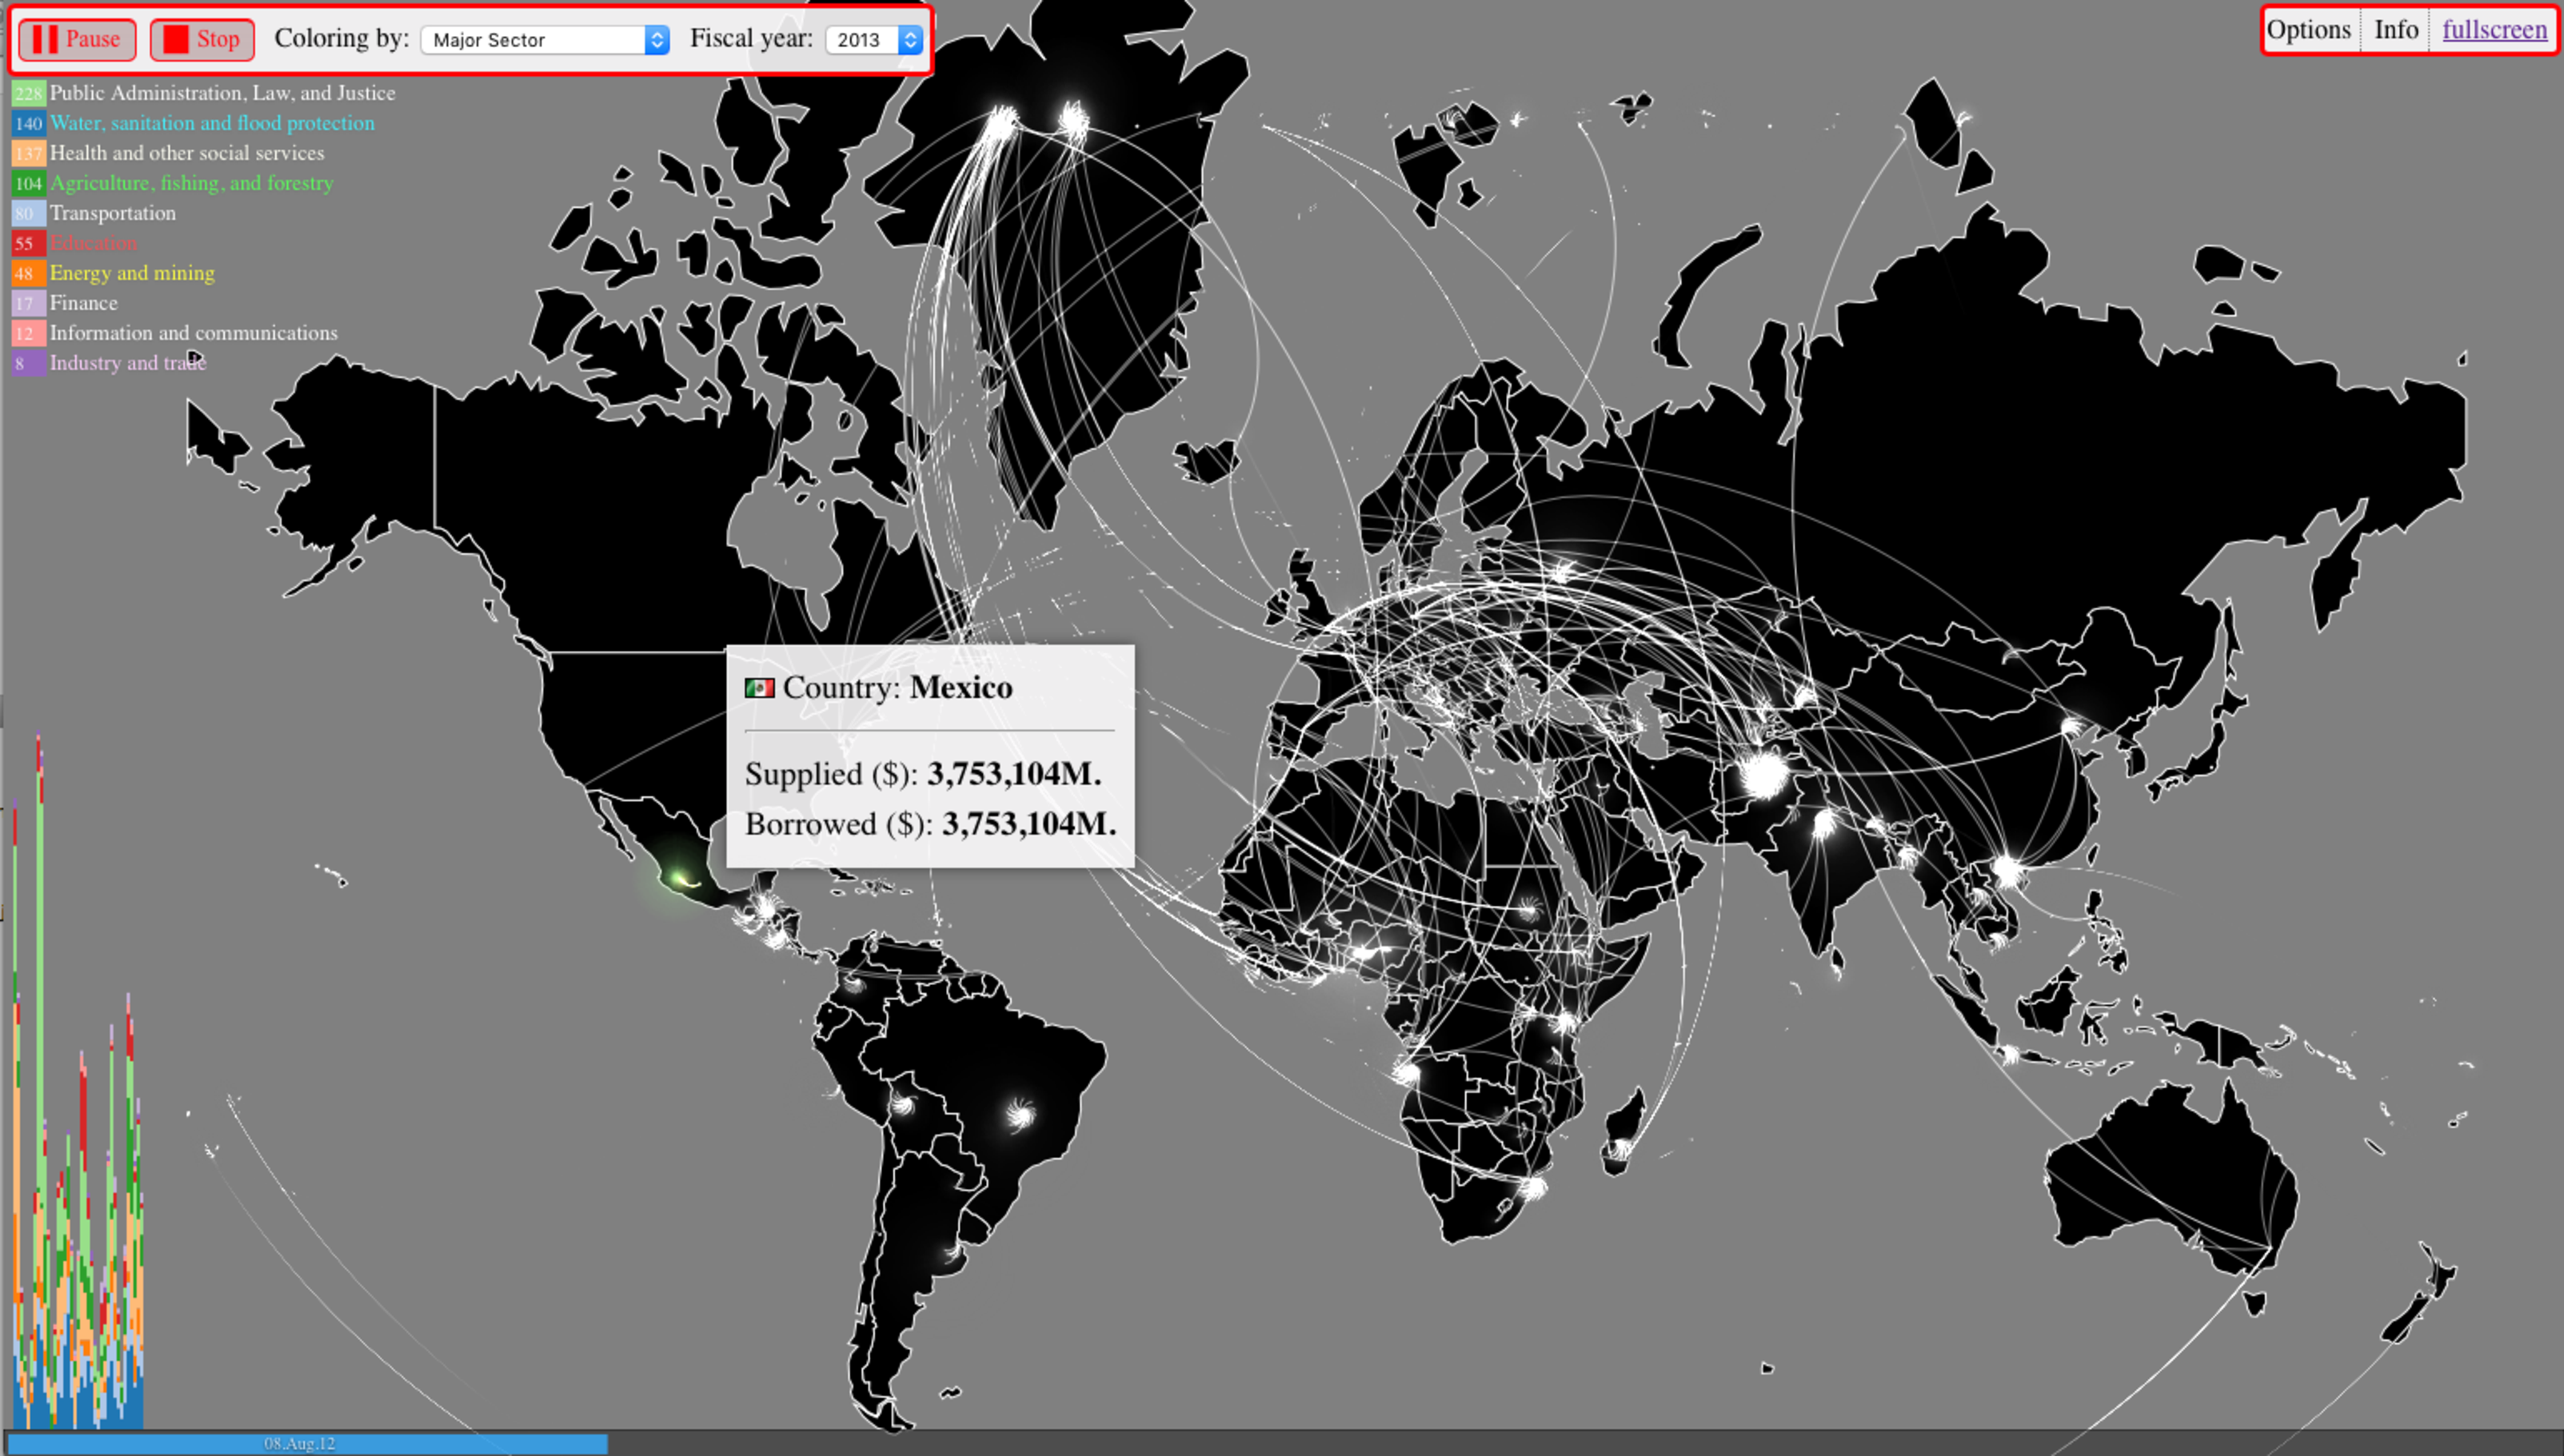
\includegraphics[width=\textwidth,height=1\textheight,keepaspectratio]{../img/interactive_map_mex.pdf}
\end{center}
\noindent \footnotesize{\textbf{Source:} Own creation based on \cite{wb_i_map}. \\Go to \href{http://detecting-corruption.carlospetricioli.com/interactive_map}{detecting-corruption.carlospetricioli.com/interactive\_map} to see a live version. \\Data from the World Bank \parencite{wb_data}.}
\end{figure}

\subsection{Companies \& projects network}

\subsection{Contract specific risk map}

\begin{figure}[H]
\begin{center}
\caption{Risk map (Sample)}
\label{fig_risk_map}
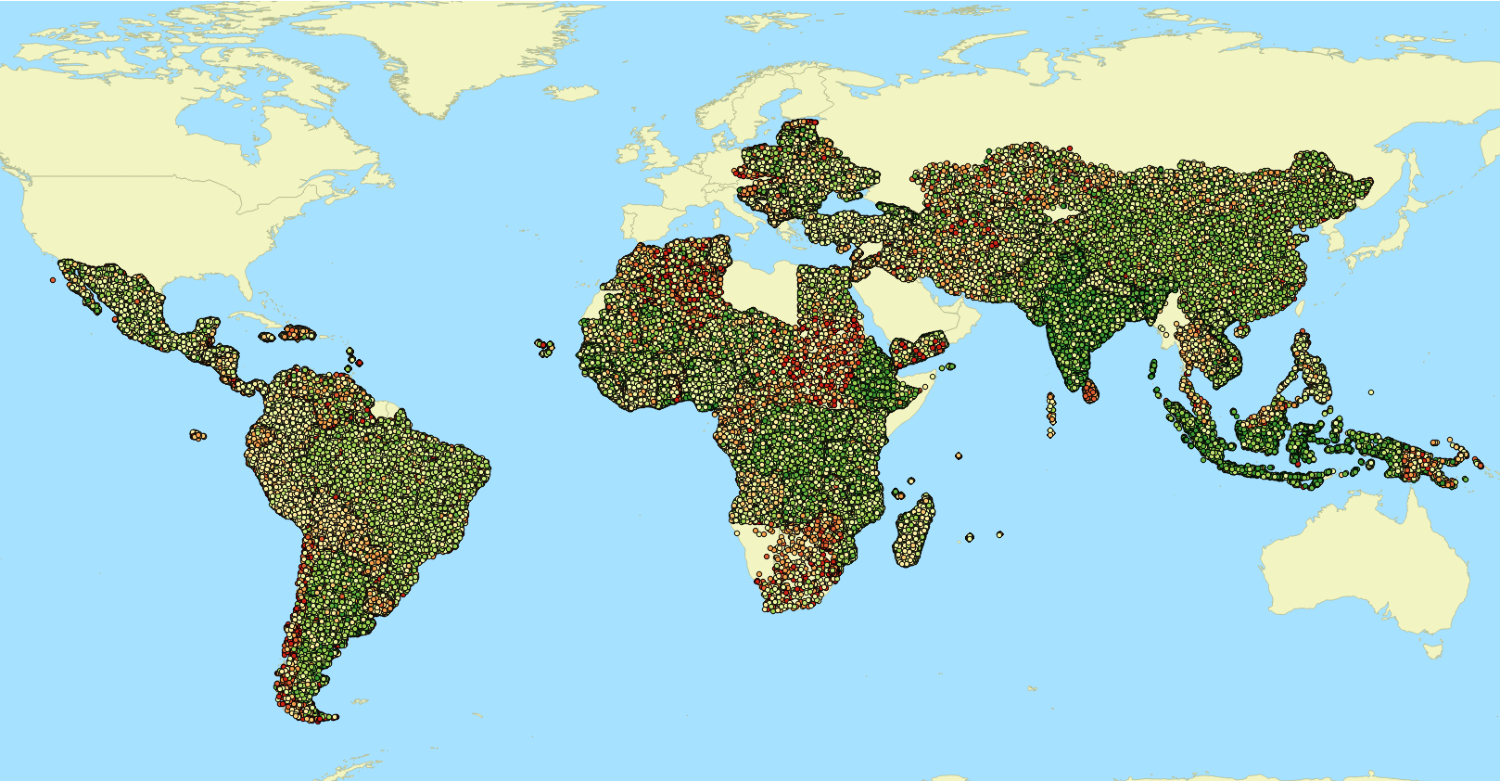
\includegraphics[width=\textwidth,height=1\textheight,keepaspectratio]{../img/risk_map.pdf}
\end{center}
\noindent \footnotesize{\textbf{Source:} Own creation based on \cite{wb_i_map}. \\Data from the World Bank \parencite{wb_data}.}
\end{figure}

